\chapter{Introduction}

\label{chapter:introduction}

In this chapter, we introduce this thesis by presenting its motivation,
describing our research questions and providing an overview of the thesis
structure.

\section{Motivation}

With the recent trend of increasingly large deep learning models achieving
state-of-the-art performance on a myriad of \ac{ml} tasks including in \ac{nlp}
as shown in Figure \ref{fig:nlp_progress}, several studies argue for focused
research into \ac{xai} to address emerging concerns such as security risks and
inductive biases associated with black-box models
\citep{doran2017does,townsend2019extracting,danilevsky2020survey,arrieta2020explainable}.
Of these studies, \citet{arrieta2020explainable} provide an extensive overview
of \ac{xai} and related concepts based on a thorough literature review of
$\sim$400 \ac{xai} research contributions published to date. In particular,
\citet{arrieta2020explainable} explore and classify a variety of
machine-learning models into transparent and black-box categories depending on
their degrees of transparency. Furthermore, they explore taxonomies of post-hoc
explainability techniques aimed at effectively explaining black-box models.
Notable explainability techniques used in recent research include local
explanations, feature relevance and explanations by simplification.

Through our own survey of recent literature on explainability techniques used in
\ac{nlp}, we came across several interesting studies employing the three
aforementioned post-hoc explainability techniques to better explain black-box
models; particularly deep neural networks.
\citep{schwartz2018sopa,peng2018rational,suresh-etal-2019-distilling,wang2019state,jiang2020cold}.
Of these studies, we draw inspiration from \citet{schwartz2018sopa} who
developed the novel hybridized \ac{rnn}, \ac{cnn} and weighted finite-state
\textbf{So}ft \textbf{Pa}tterns (SoPa) model architecture with a special focus
in model explainability. While the SoPa model functions well, we found its
explainability techniques to be localized and indirect despite its weighted
finite-state components providing a strong potential for effective explanations
by simplification into a transparent and global regular-expression-based model.
The main objective of this thesis is to address these limitations and
to propose a modified model, \textbf{SoPa++}, which could allow for effective
explanations by simplification. To facilitate this objective, we evaluate the
performance and explanations by simplification of the modified SoPa++ model on
the recently released \ac{fmtod} data set from
\citet{schuster-etal-2019-cross-lingual}; focusing on the English-language
intent classification task.

\begin{figure}[t!]
  \centering
  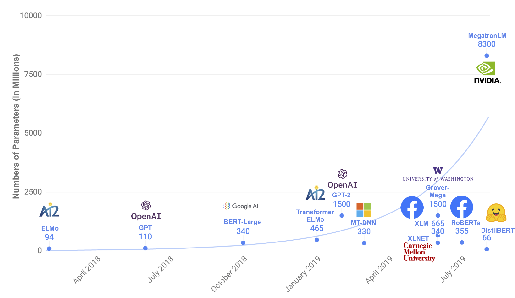
\includegraphics[width=13cm]{pdfs/borrowed/nlp_sota_model_size_progress.pdf}
  \caption{Parameter counts of recently released pre-trained language models
    which showed competitive or state-of-the-art performance when fine-tuned
    over a range of NLP tasks; figure taken from \citet{sanh2019distilbert}}
  \label{fig:nlp_progress}
\end{figure}

\section{Research questions}

\label{section:rq}

To guide us in addressing our objective, we aim to answer the following three
research questions:

\begin{enumerate}
  \item Does SoPa++ contribute to competitive performance\footnote{We define
    competitive performance as the scenario where a mean performance metric on a
    certain task falls within the range obtained from other recent studies on
    the same task} on the \ac{fmtod} English language intent classification task?
  \item To what extent does SoPa++ contribute to effective explanations by
  simplification on the \ac{fmtod} English language intent classification task?
  \item What interesting and relevant explanations can SoPa++ provide on the
  \ac{fmtod} English language intent classification task?
\end{enumerate}

\section{Thesis structure}

We now summarize the contents and structure of this thesis.

\begin{description}[align=left]
  \item [Chapter \ref{chapter:introduction}:] Introduce this thesis, its
  contents and our research questions.
  \item [Chapter \ref{chapter:background}:] Describe the background concepts
  utilized in this thesis.
  \item [Chapter \ref{chapter:methodologies}:] Describe the \ac{fmtod} data set and
  methodologies pursued in this thesis.
  \item [Chapter \ref{chapter:results}:] Describe the results obtained from our
  methodologies.
  \item [Chapter \ref{chapter:discussion}:] Interpret the results and discuss their
  implications.
  \item [Chapter \ref{chapter:conclusions}:] Summarize and conclude the findings
  of this thesis.
  \item [Chapter \ref{chapter:further_work}:] Describe future work to expand on
  our research questions.
\end{description}

%%% Local Variables: 
%%% mode: latex
%%% TeX-master: "main"
%%% End: 